\documentclass{article}
\usepackage[a4paper, total={6in,9in}]{geometry}
\usepackage{fancyhdr}
\usepackage{graphicx}
\usepackage{tcolorbox}
\usepackage{hyperref}
\usepackage{listings}
\begin{document}
\pagestyle{fancy}
\fancyhead[L]{CURI Pre-interview}

\section*{Introduction}
Hello! This is Professor Leeson. 
If you are reading this document, then that means you have shown interest in working with me over the summer and I have offered you an interview.
If this is not the case, I'm not quite sure how you got this.

I am personally not a huge fan of coding interviews. 
I very much value the ability to work independently and problem solving.
It's hard to identify these skills in a coding interview where you are put on the spot.
Most of the times, it just shows the ability to memorize problems.
In lieu of a coding interview, I am asking you to work on the tasks I present in this write-up.
These tasks will be related to the work we will be doing over the summer.
These tasks can be completed on the lab machines in RNS 202 and 203.
Feel free to SSH into them using VSCode and a terminal.
During the interview, we will discuss your process, what problems you faced, how you tried to overcome then, etc.

I would like to emphasize that you do not need to complete all of the tasks.
It's quite possible you will reach a point you are not sure how to get past.
That is ok.
What is important is that you investigate the problem and come to the interview willing to talk about it.
I would suggest you work for at max 4 hours in total on these tasks.
I acknowledge that this is during the semester where you have other responsibilities, so to ask more would be unrealistic.
Do your best and come ready to talk about what you did.

In the process of solving these tasks, you will almost certainly write some code.
Please come to the interview ready to discuss the code you wrote.
You are allowed to use outside sources, such as StackOverflow, ChatGPT, a professor from MIT, etc.
However, you will be expected to know what all of your code does.
Be ready to explain it as I might ask questions during the interview.

\section*{Task 1 - Getting a Repo Set-up}
The first thing I would like you to do is fork the ``pre-interview'' repository.
It is located at \url{https://github.com/will-leeson/pre-interview}.
To do so, you will need to have a Github account.
If you don't have one, now would be a great time to make one. 
Github is used a lot in computer science.
Github requires you to use SSH keys to download and push to repositories, so you will need to set those up like you did for CSGit.
Here is a nice tutorial: \href{https://docs.github.com/en/authentication/connecting-to-github-with-ssh/generating-a-new-ssh-key-and-adding-it-to-the-ssh-agent}{SSH Key Github Tutorial}.
Once you have a github account you need to create a ``fork'' of this repository.
A fork is basically like taking another git repository and branching off of it to make a new repository.
Once you have forked the repository, clone it and invite me to your repo (my github username is will-leeson).
In the README file, please put your name and one fun fact about you.

\section*{Task 2 - Getting an SMT solver running on your machine}
For these the following tasks, you will need to be able to run an SMT solver.
There are tons of them.
You can use any one you like, but I suggest using CVC5.
Its a great SMT solver and they provide precompiled binaries for many types of computers.
Here is a link to the latest version \url{https://github.com/cvc5/cvc5/releases/tag/cvc5-1.2.1}.
On this page they have a series of ``assets'' which include compressed versions of the precompiled solver.
If you are using one of the machines in RNS 202/203 (either in person of via SSH), you should download "cvc5-Linux-arm64-static.zip".
If you are using your own machine, they name the binaries according to the machine it is built for. I suggest you use a static build.
To download a file from the internet to a machine via command line, you can use the ``wget'' command.

Once you have downloaded the tool, extract it. In a terminal, you can extract a zip file with the ``unzip'' command. You should now have a folder ``cvc5-Linux-x86\_64-static''.
Inside it, you should see the following files/folders: AUTHORS, bin, COPYING, include, lib, licenses.
Inside the bin folder is a binary executable called cvc5.
This is the SMT solver.
We can run the binary to check it is working by running the executable with the ``-{}-version'' option.
From the bin folder, run the following command: \texttt{./cvc5 -{}-version}. You should see something like this:
\newpage
\begin{figure}[!t]
    \centering
    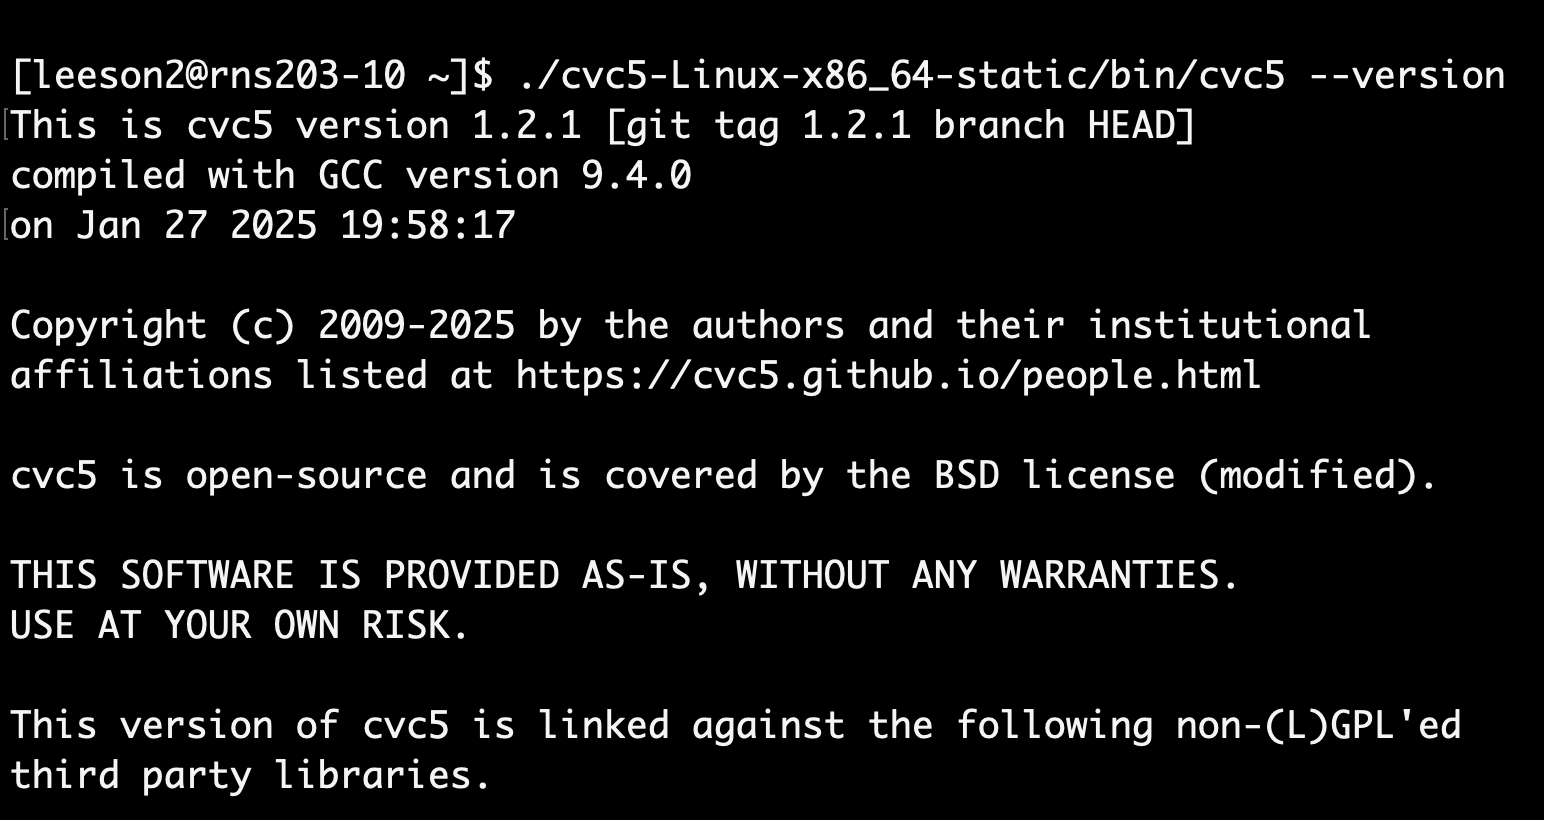
\includegraphics[width=0.9\textwidth ]{imgs/CVC-version.png}
    \caption{CVC5 version command output}\label{fig:CVC5-version}
\end{figure}

You can then run CVC5 on an SMT file like this: \texttt{./cvc5 [/path/to/file]}, where file is an SMT file. I have provided some sample queries in the repository in the queries folder. I ran it on the query ``up\_reach\_Query33.smt2'' and got the following output:

\begin{figure}[!h]
    \centering
    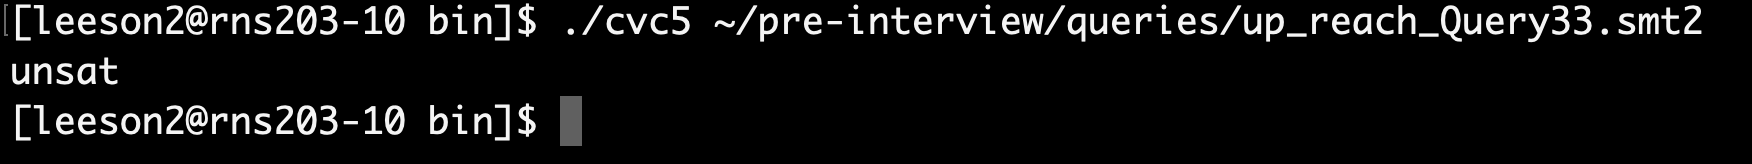
\includegraphics[width=0.9\textwidth ]{imgs/CVC-Running.png}
    \caption{Running CVC5}\label{fig:CVC5-running}
\end{figure}

\noindent
I guess that query is unsatisfiable. Cool!

\section*{Task 2b - Time Out}
The SMT files provided in the ``queries'' folder range in difficulty. Some might take quite a while.
To ensure we aren't waiting forever, we can tell CVC5 to enforce a time out.
This means, when a certain amount of time has elapsed, the solver will stop and report it couldn't finish.
Figure out how to put a 1 minute timeout on CVC5.
Run CVC5 on each query using this timeout value and record if they were SAT, UNSAT, or if the timed out.

\section*{Task 3 - Running the Solver on Several Queries}
Now that you got a solver working, we can run it on a bunch of problems, which is what we'll be doing over the summer.
Running the solver on each query is time consuming and doing it manually is a waste, especially when there are thousands of problems.
Instead, we can write a program to do it for us.
Generally, this type of program is called a ``script''.
Scripts are typically a small, single file program that does a task for you.
Popular ``scripting'' languages include Python, JavaScript, or Shell.

For this task, I want you to write a script that will automate the process of running the SMT solver on a lot of queries.
The script should take a folder in as input, like the folder of queries I have provided.
This way, you can run the script, go grab a bite to eat, and when you're back, all of the queries will have been run.
I don't care what language you write this script in.
Choose whatever you are most comfortable with.
I wrote my script using Shell, but any language should be able to handle this fine.
Shell is nice because you can essentially copy terminal commands you would run.
The end result should be a file called ``run-queries.[ext]'' where ext is the appropriate file extension for the language you choose.
In the README file in this repository, please explain how to run your code.
Whatever code you end up writing, please push it to your fork of this repository, even if it is incomplete.

\section*{Task 4 - Collecting Data}
Once you have a script that can run the queries, we need to be able to collect some data from them. In particular, we care about if it was satisfiable or not and how long it took to run.
Create a program that will take the results from running each query and produce a CSV file where each line is formatted as follows:

\vspace{2mm}
\noindent
QueryName,Result,ElapsedTime
\vspace{2mm}

\noindent
QueryName should be the file name of the query.
Result should be SAT/UNSAT/TIMEOUT.
ElapsedTime should be the time it took to run.
The program which produces the file could be the same script you used to run the queries. 
Or, you can alter your prior script to record the raw data, and then write another script to parse it. It's up to you!
Just update the README to explain how to run your code.
Make sure to push your code!

\section*{Task 5 - Bask in the glow of your achievements}
Great job! Please make sure to push any code you wrote and explanations for how to run it in the README. Remember, I don't expect you to have complete all tasks for the interview. Just get as far as you can.

\end{document}